\documentclass[12pt,english]{article}

\usepackage[a4paper,
bindingoffset=0.2in,
left=1in,
right=1in,
top=1in,
bottom=1in,
footskip=.25in]{geometry}

\usepackage{graphicx}
\usepackage{makecell}
%================================

\newlength{\resLen}
\setlength{\resLen}{1.7in}

\begin{document}
		
	% In the middle if you want to change the margins use
	\newgeometry{left=0.35in,right=0.35in,top=0.5in,bottom=0.5in}

	\begin{center}
		\LARGE\textbf{Previous Projects (main contribution)}
	\end{center}
	
	\Large\textbf{Tencent America:}
	\begin{figure}[h]
		\textbf{
		\begin{tabular}{p{\resLen}p{\resLen}p{\resLen}p{\resLen}}
			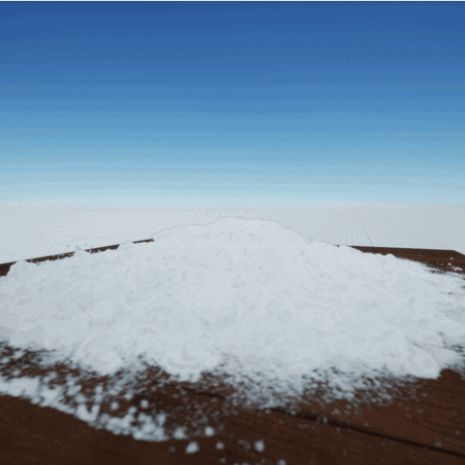
\includegraphics[height=\resLen]{snow.jpg} &
			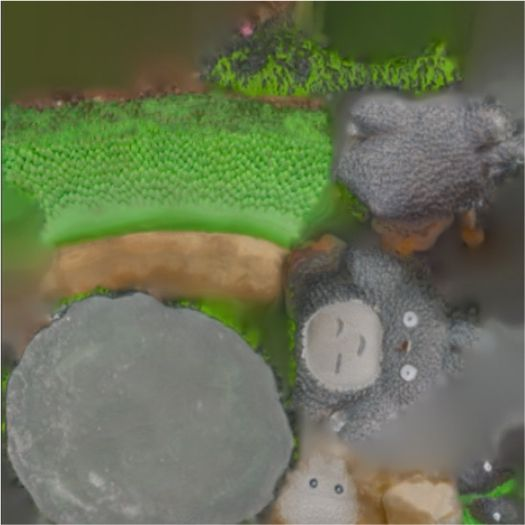
\includegraphics[height=\resLen]{delight.jpg} &
			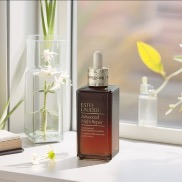
\includegraphics[height=\resLen]{realitybooth.jpg} &
			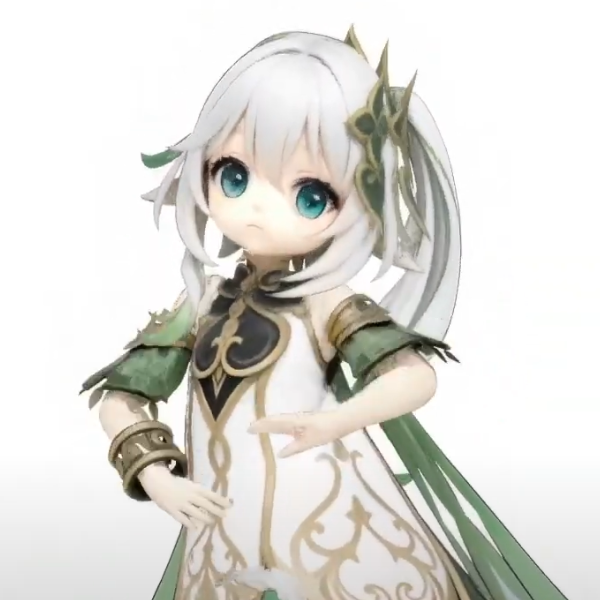
\includegraphics[height=\resLen]{genshin.png} \\
			- UE5 plugin               & - Photogrammetry  & - Image generation & - Cartoon stylization \\
			- Snow rendering & - Texture delighting             & - Diffusion models & - Stable Diffusion \\
			- Multiple scattering &  - Shadow removal  & - Relighting & - Video stabilization
		\end{tabular}}
	\end{figure}

	\Large\textbf{During PhD:}
	\begin{figure}[h]
		\textbf{
		\begin{tabular}{p{\resLen}p{\resLen}p{\resLen}p{\resLen}}
			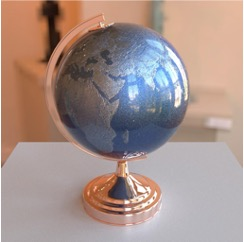
\includegraphics[height=\resLen]{layer.jpg} &
			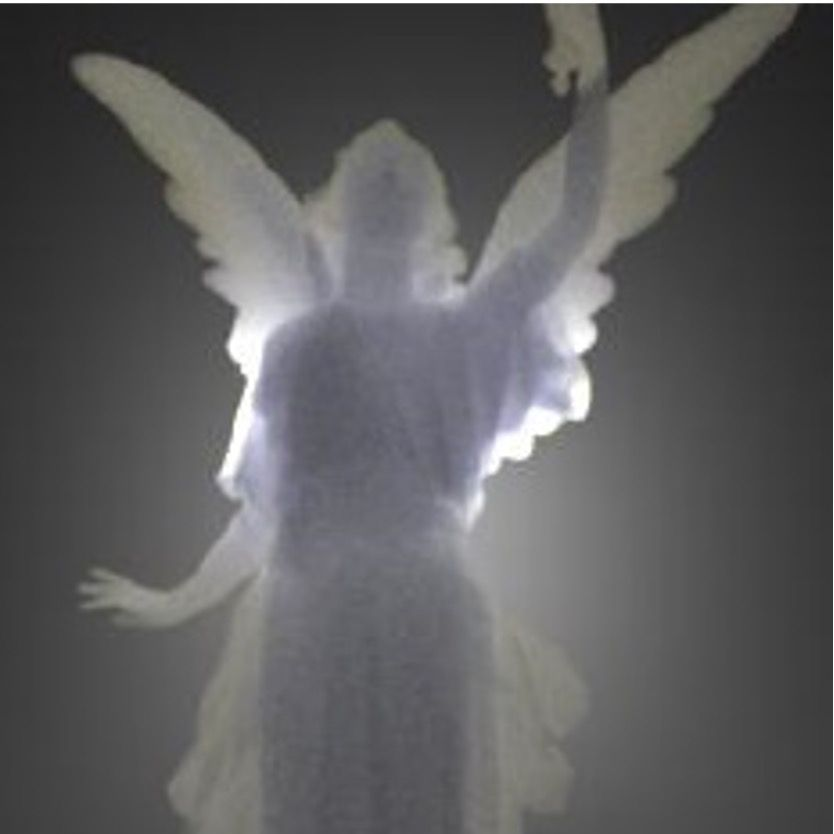
\includegraphics[height=\resLen]{waveoptics.jpg} &
			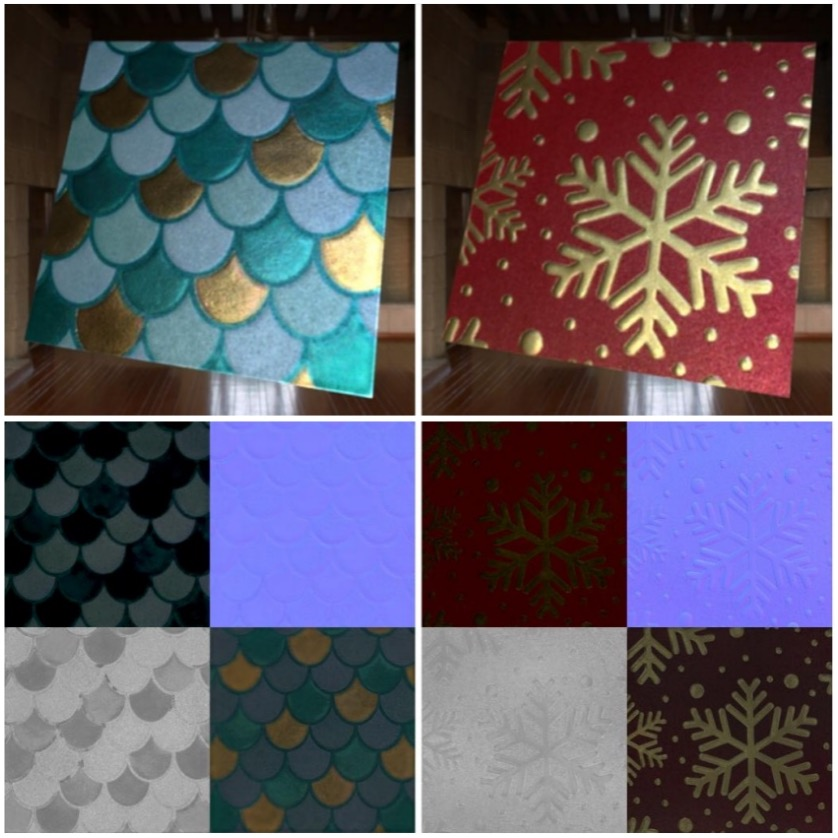
\includegraphics[height=\resLen]{materiangan.jpg} &
			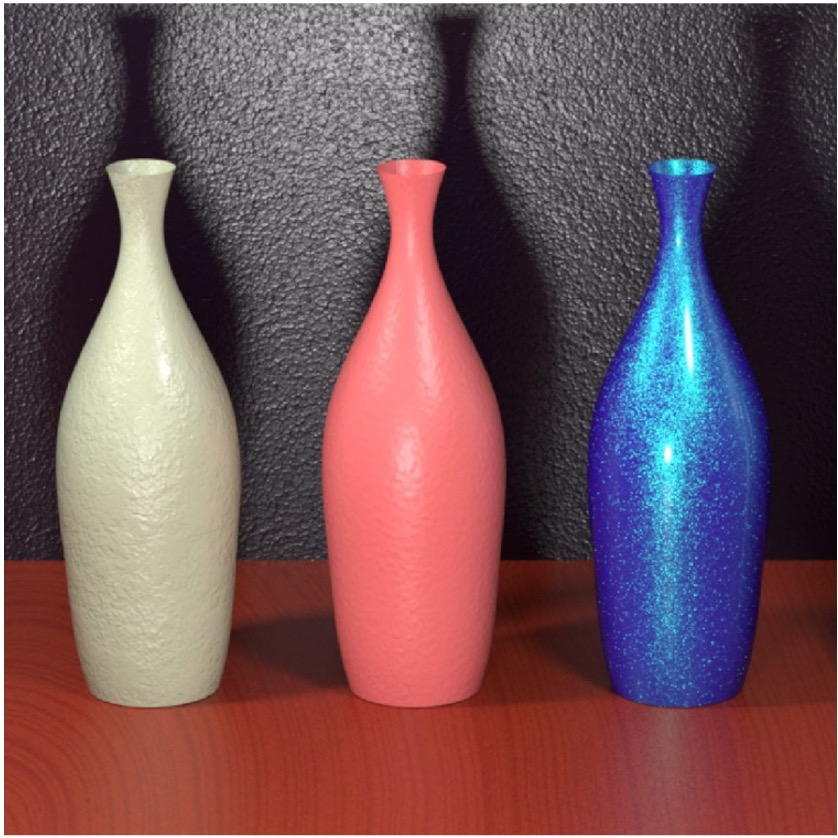
\includegraphics[height=\resLen]{bayesian.jpg} \\
			- Forward rendering & - Volume rendering & - Inverse-rendering & - \small{Procedural material} \\
			- Layered BSDF        & - Wave optics                            & - SVBRDF                  & - Bayesian theory \\
			- PBRT-v4                 &                                                     & - MaterialGAN           & - MCMC sampling
		\end{tabular}}
	\end{figure}
	
	\Large\textbf{Human face related:}
	\begin{figure}[h]
		\textbf{
		\begin{tabular}{p{\resLen}p{\resLen}p{\resLen}}
			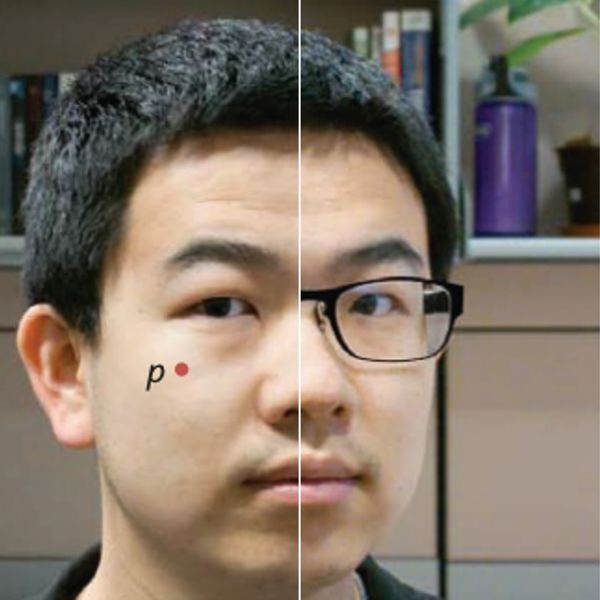
\includegraphics[height=\resLen]{glasses.jpg} &
			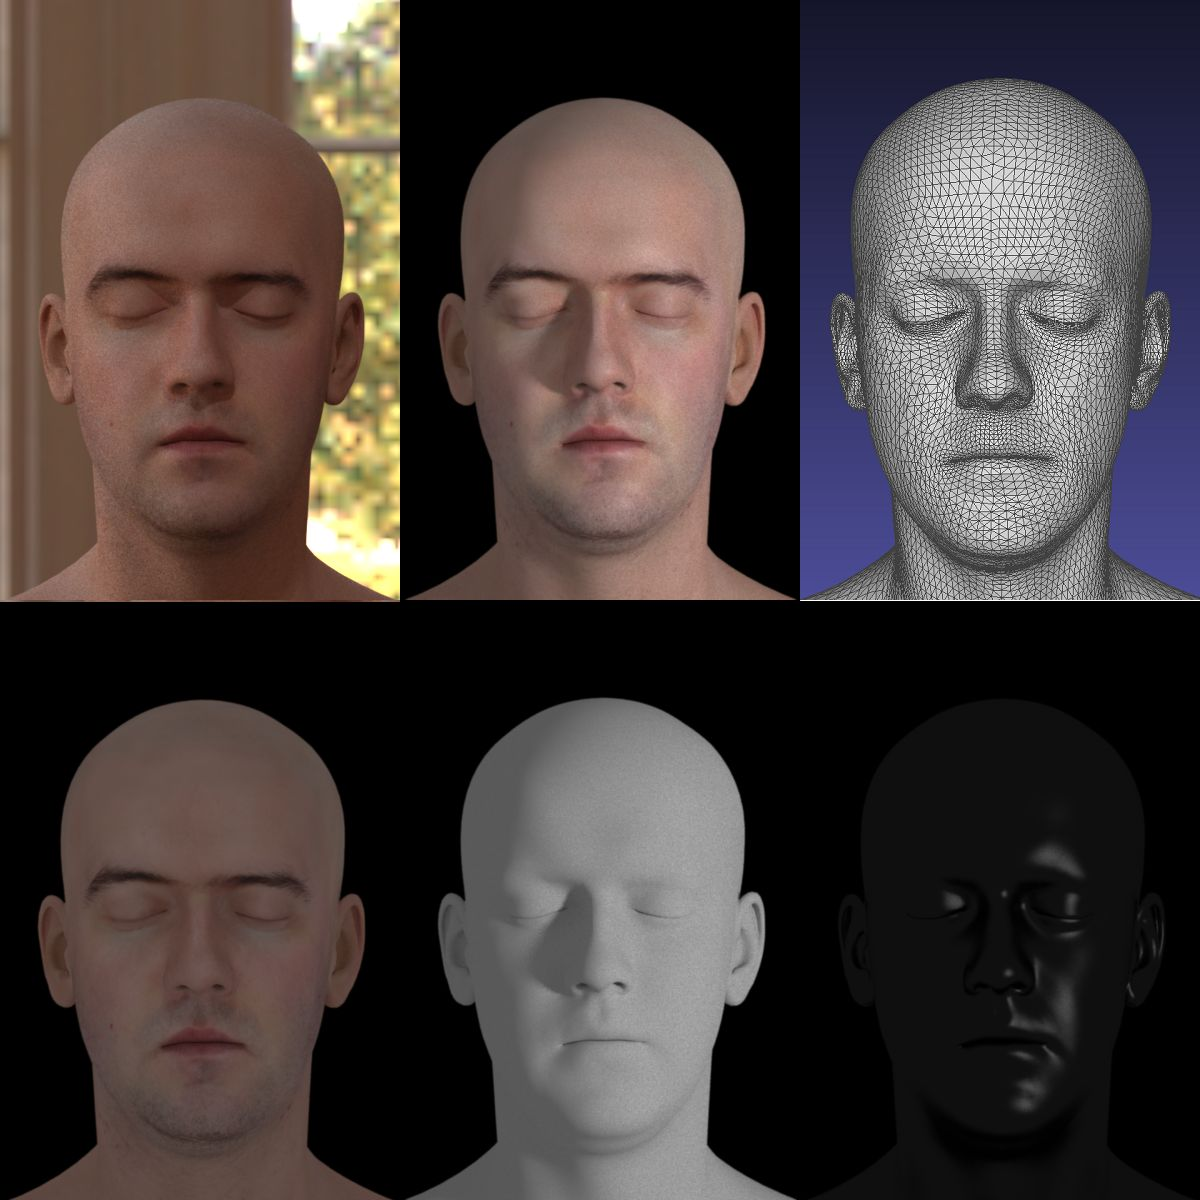
\includegraphics[height=\resLen]{face.jpg} &
			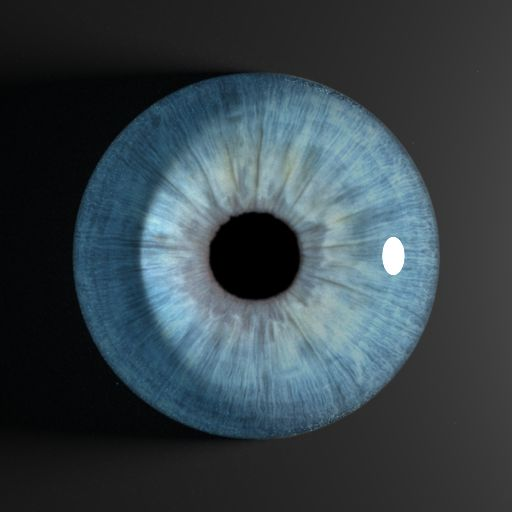
\includegraphics[height=\resLen]{eye.jpg} \\
			- Virtual try-on             & - Face relighting  & - Eye rendering \\
			- Prescription glasses & - Face rendering  & - Eye reconstruction \\
		\end{tabular}}
	\end{figure}
	
	%to restore old margins, use
	\restoregeometry
		
\end{document}
	